\subsection{Case05 - Broadcast}
\label{p4_wifi_case05}


En este test desarrollaremos un programa p4 que haga Broadcast. En este caso únicamente haremos Broadcast a nivel de enlace, capa 2. La motivación de este caso de uso es ver la diferencia de dificultad respecto del entorno XDP donde tuvimos que anclar de manera adicional un \textit{bytecode} e\gls{bpf} en el \gls{tc} además de propio programa \gls{xdp} anclado en la interfaz para lograr hacer un broadcast. Al igual que en los casos de uso anteriores, se hará uso de software switch llamado \gls{bmv2}, para testear los programas P4, y de la integración desarrollada anteriormente con Mininet-WiFi como escenario para recrear las topologías de Red.\\
\par


Dado que toda la información relativa a este caso de uso ya se ha explicado anteriormente en el case05 de P4 cableado (Ver subsección \ref{P4_ether_case05}), y no hay ninguna diferencia inducida en el cambio de entorno según se explico en las sección anterior,  únicamente se harán indicaciones sobre como poder compilarlo y ejecutarlo. Importante, como ya se ha indicado, si usted está replicando este caso de uso, sin antes haber adecuado las dependencias necesarias de Mininet-WiFi con soporte del \gls{bmv2}, vuelva a este punto \ref{mn_wifi_own_deps} y siga los pasos indicados.

% figura escenario
\begin{figure}[ht]
    \centering
    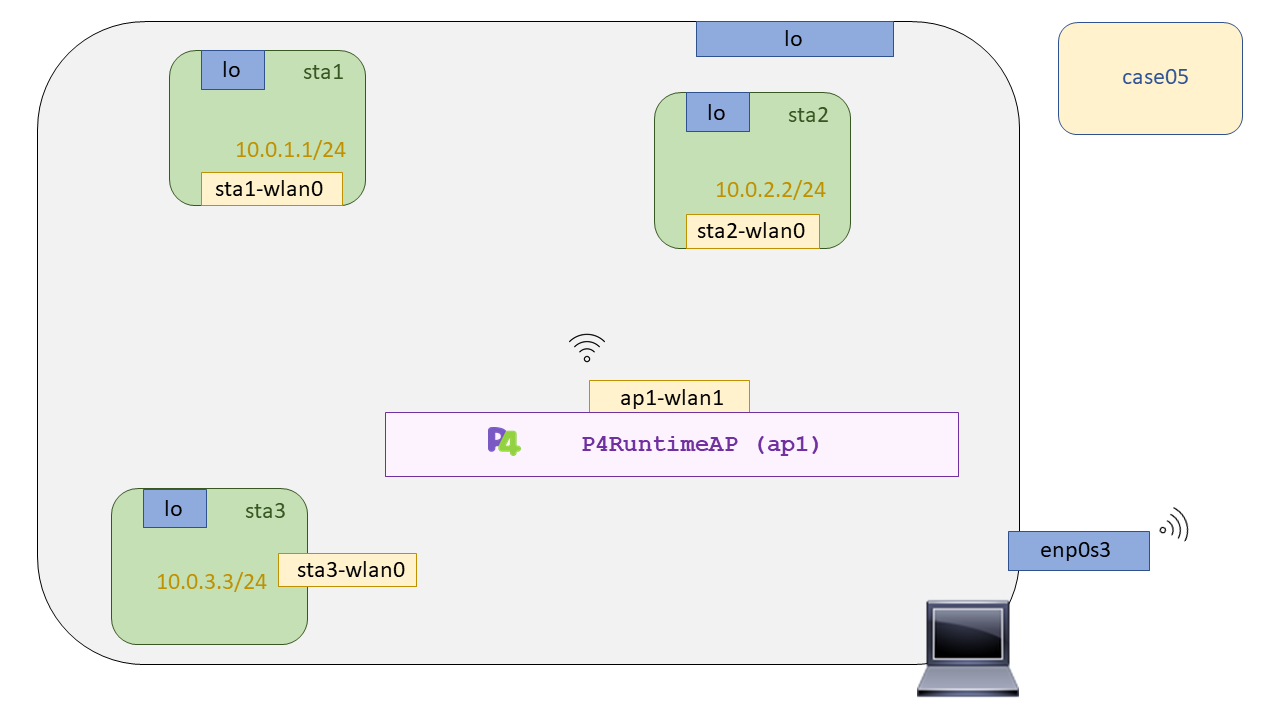
\includegraphics[width=16cm]{archivos/img/dev/p4-wifi/case05/scenario.png}
    \caption{Escenario del Case05 - P4 Wireless}
    \label{fig:case05_p4_wifi_scenario}
\end{figure}

\newpage

\vspace{0.2cm}
\textbf{Compilación}\\
\par

Para la compilación de este caso de uso, al igual que en los casos de uso anteriores se ha dejado preparado un Makefile, por tanto no es necesario que el usuario haga un uso directo del compilador p4c. Si se quiere saber más sobre como funciona el proceso de compilación, qué etapas hay, como se le "inyecta" el \texttt{json} generado al \gls{bmv2}, o qué distintos \textit{targets} hay en función de la arquitectura, le recomendamos que vuelva al case01 (\ref{p4_ether_case01}). Para llevar a cabo la compilación solo se tendrá que seguir los pasos indicados en el bloque \ref{code:case04_p4_wifi_load}.

\begin{lstlisting}[language= bash, style=Consola, caption={Compilación programa P4  - Case05},label=code:case05_p4_wifi_load]
    # Entramos al directorio 
    cd TFG/src/use_cases/p4-wireless/case05

    # Hacemos uso del Makefile
    sudo make
\end{lstlisting}
\vspace{0.5cm}


Una vez ejecutado el make, se habrá generado una estructura de directorios que se utilizarán en el lanzamiento del caso de uso. Bajo el directorio \texttt{build} se podrá encontrar el \texttt{json} generado por el compilador, será este \texttt{json} quien tenga toda la información requerida para conformar el \gls{bmv2}. Los directorios \texttt{log} y \texttt{pcap}, se utilizarán respectivamente para almacenar los logs del \gls{bmv2} y para guardar las capturas de paquetes de las interfaces asociadas a la instancia \gls{bmv2}.\\
\par



\vspace{0.2cm}
\textbf{Puesta en marcha del escenario}\\
\par

Al igual que en la compilación, se ha suministrado un script en Python para automatizar la puesta en marcha del escenario. Este script conformará la topología que se utilizará en este caso de uso. Se quiere recordar que es necesario volver hacer un \texttt{make install} para instalar los módulos adicionales generados para la integración del \gls{bmv2} y Mininet-WiFi, además de tener instaladas las versiones indicadas en el análisis de la integración. Estas dependencias se pueden encontrar en el apartado \ref{mn_wifi_own_deps} \\
\par

Una vez comprobadas la dependencias, simplemente se tendrá que ejecutar el script con el interprete de Python. Este script levantará la topología descrita en la figura \ref{fig:case05_p4_wifi_scenario}, compuesto por tres estaciones WiFi y por una instancia del nodo \texttt{P4RuntimeAP}. El nodo \texttt{ap1}, del tipo \texttt{P4RuntimeAP}, tendrá una interfaz,  del tipo wireless, con la cual se comunicará con todas las estaciones WiFi.



\begin{lstlisting}[language= bash, style=Consola, caption={Puesta en marcha del escenario  - Case05},label=code:case05_p4_wifi_run]
    sudo python scenario.py
\end{lstlisting}
\vspace{0.2cm}

\vspace{0.5cm}
\textbf{Comprobación del funcionamiento}\\
\par


Tras las ejecución del script \texttt{scenario.py}, se tendría el escenario \ref{fig:case05_p4_wifi_scenario} levantado, y la CLI de Mininet-WiFi abierta. Para la comprobación de funcionamiento de este caso de uso, se van a seguir los mismos pasos que en el case05 (\ref{P4_ether_case05}) - P4 en un entorno alámbrico. Por tanto no se entrará hacer explicaciones que se creen redundantes, se indicarán los pasos seguidos para llevar a cabo la comprobación de funcionamiento y los resultados de dichas pruebas. 

\begin{lstlisting}[language= bash, style=Consola, caption={Pasos a seguir para comprobar el funcionamiento - Case05},label=code:case05_p4_wifi_func1]
    mininet-wifi>  xterm sta1 sta2 sta3
    
    # Nos ponemos a escuchar en las estaciones wifi destino
    [sta2] tcpdump -l
    [sta3] tcpdump -l
    
    
    # Generamos ARP-Request desde sta1
    [sta1] arping 10.0.2.2
\end{lstlisting}
\vspace{0.5cm}


Como se puede apreciar en la figura \ref{fig:case05_p4_wifi_func1} el ARP-Request llega correctamente. Se ve como los paquetes ARP-Request están llegando tanto al \texttt{sta2} como a la \texttt{sta3}. Pero solo será la \texttt{sta2}, en este caso, la que contesta ya que va dirigido a ésta. \\
\par

Esto se debe a que al completarse la resolución ARP, la \texttt{sta1} ya conoce la dirección MAC de la \texttt{sta2}, por tanto los ARP-Request que se generen a posteriori llevarán la MAC destino la de la estación WiFi \texttt{sta2}, entonces el \gls{ap} no lo difundirá por todos su puertos, se lo pasará directamente a la \texttt{sta2}.

\newpage

\begin{figure}[h!]
    \centering
    \begin{subfigure}[b]{\textwidth}
    	\centering
        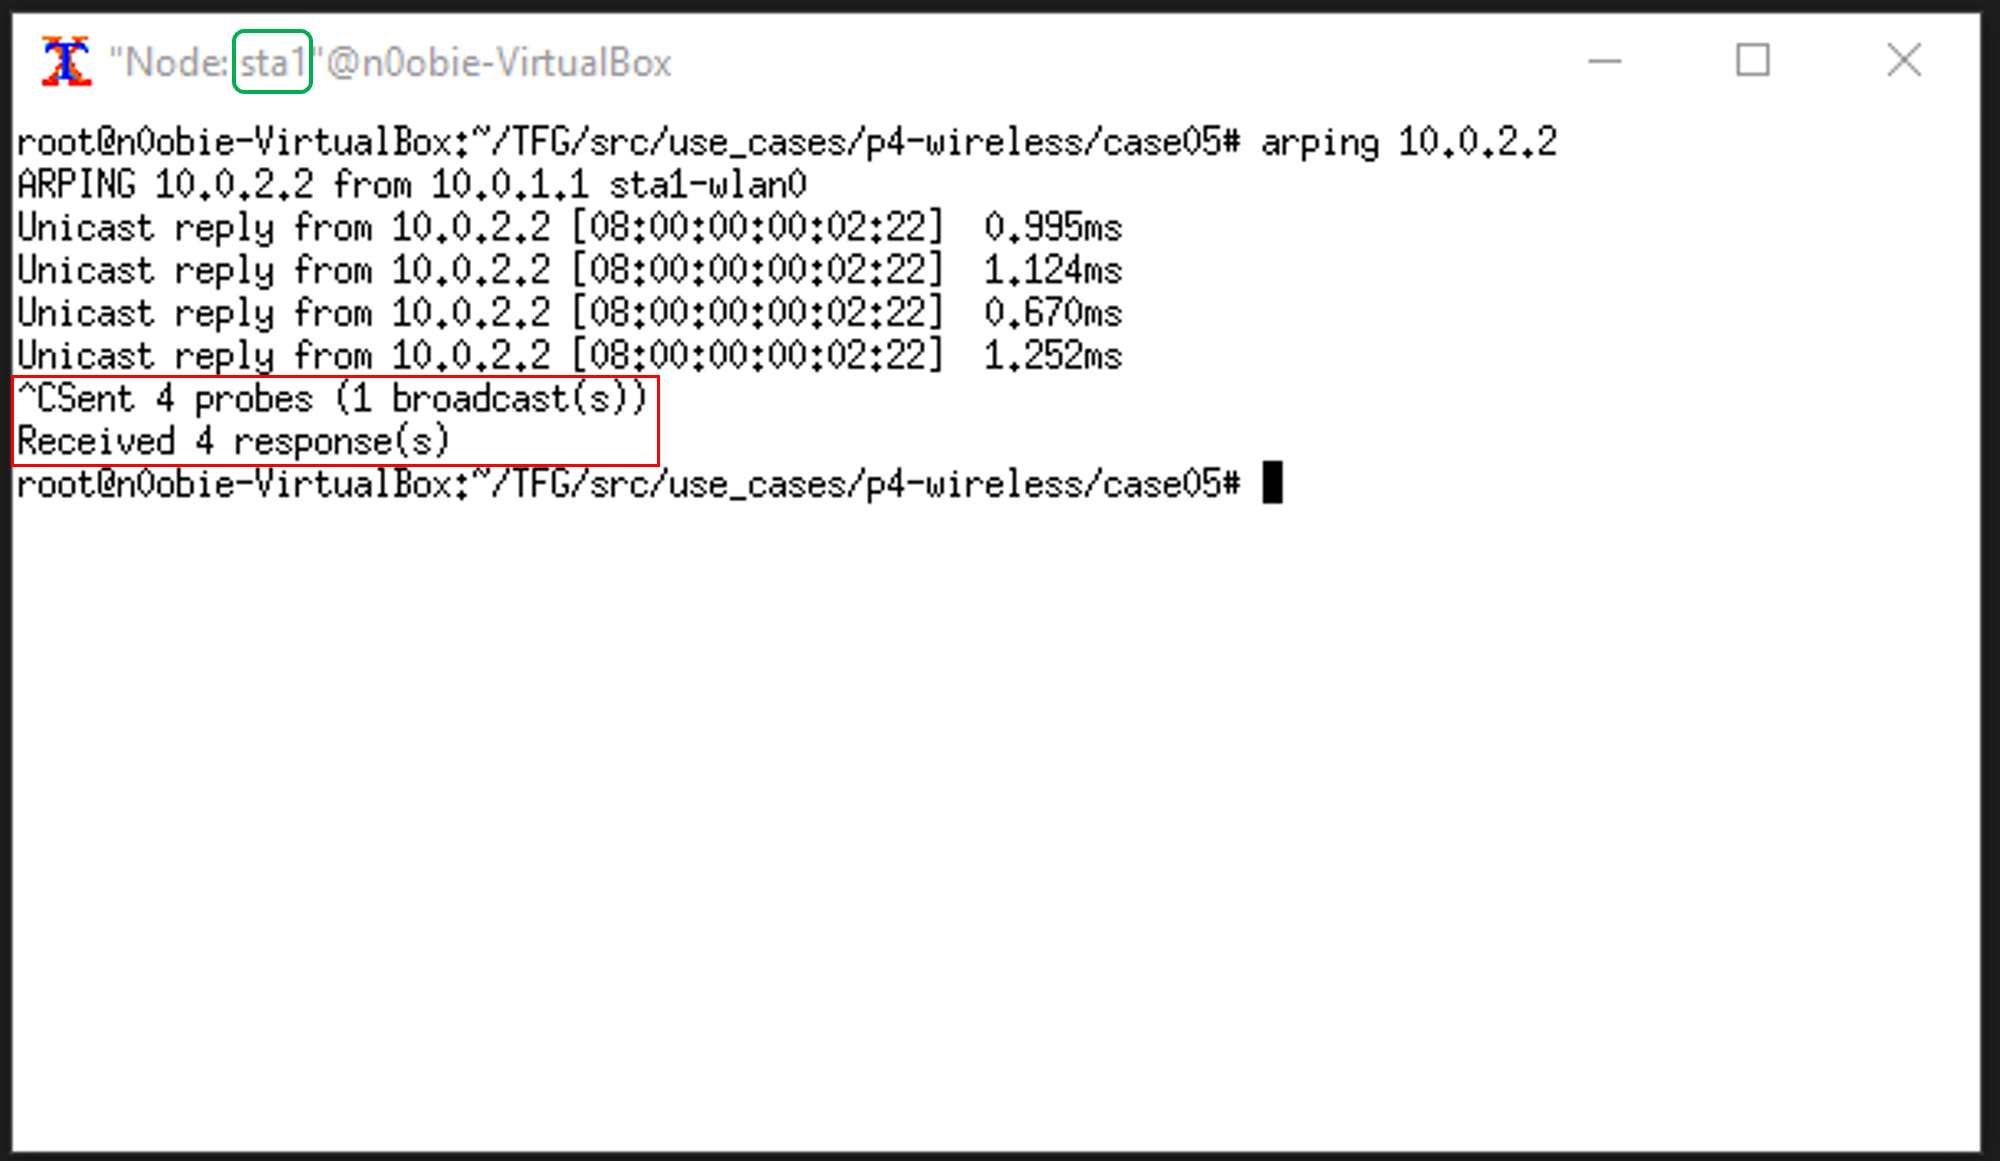
\includegraphics[width=8cm]{archivos/img/dev/p4-wifi/case05/demo_case05_1_edited.png}
        \caption{Ejecución de arping hacia la estación WiFi sta2}
        \label{fig:case05_p4_wifi_func_ping}
    \end{subfigure}
    \par\bigskip
    \begin{subfigure}[b]{\textwidth}
    	\centering
        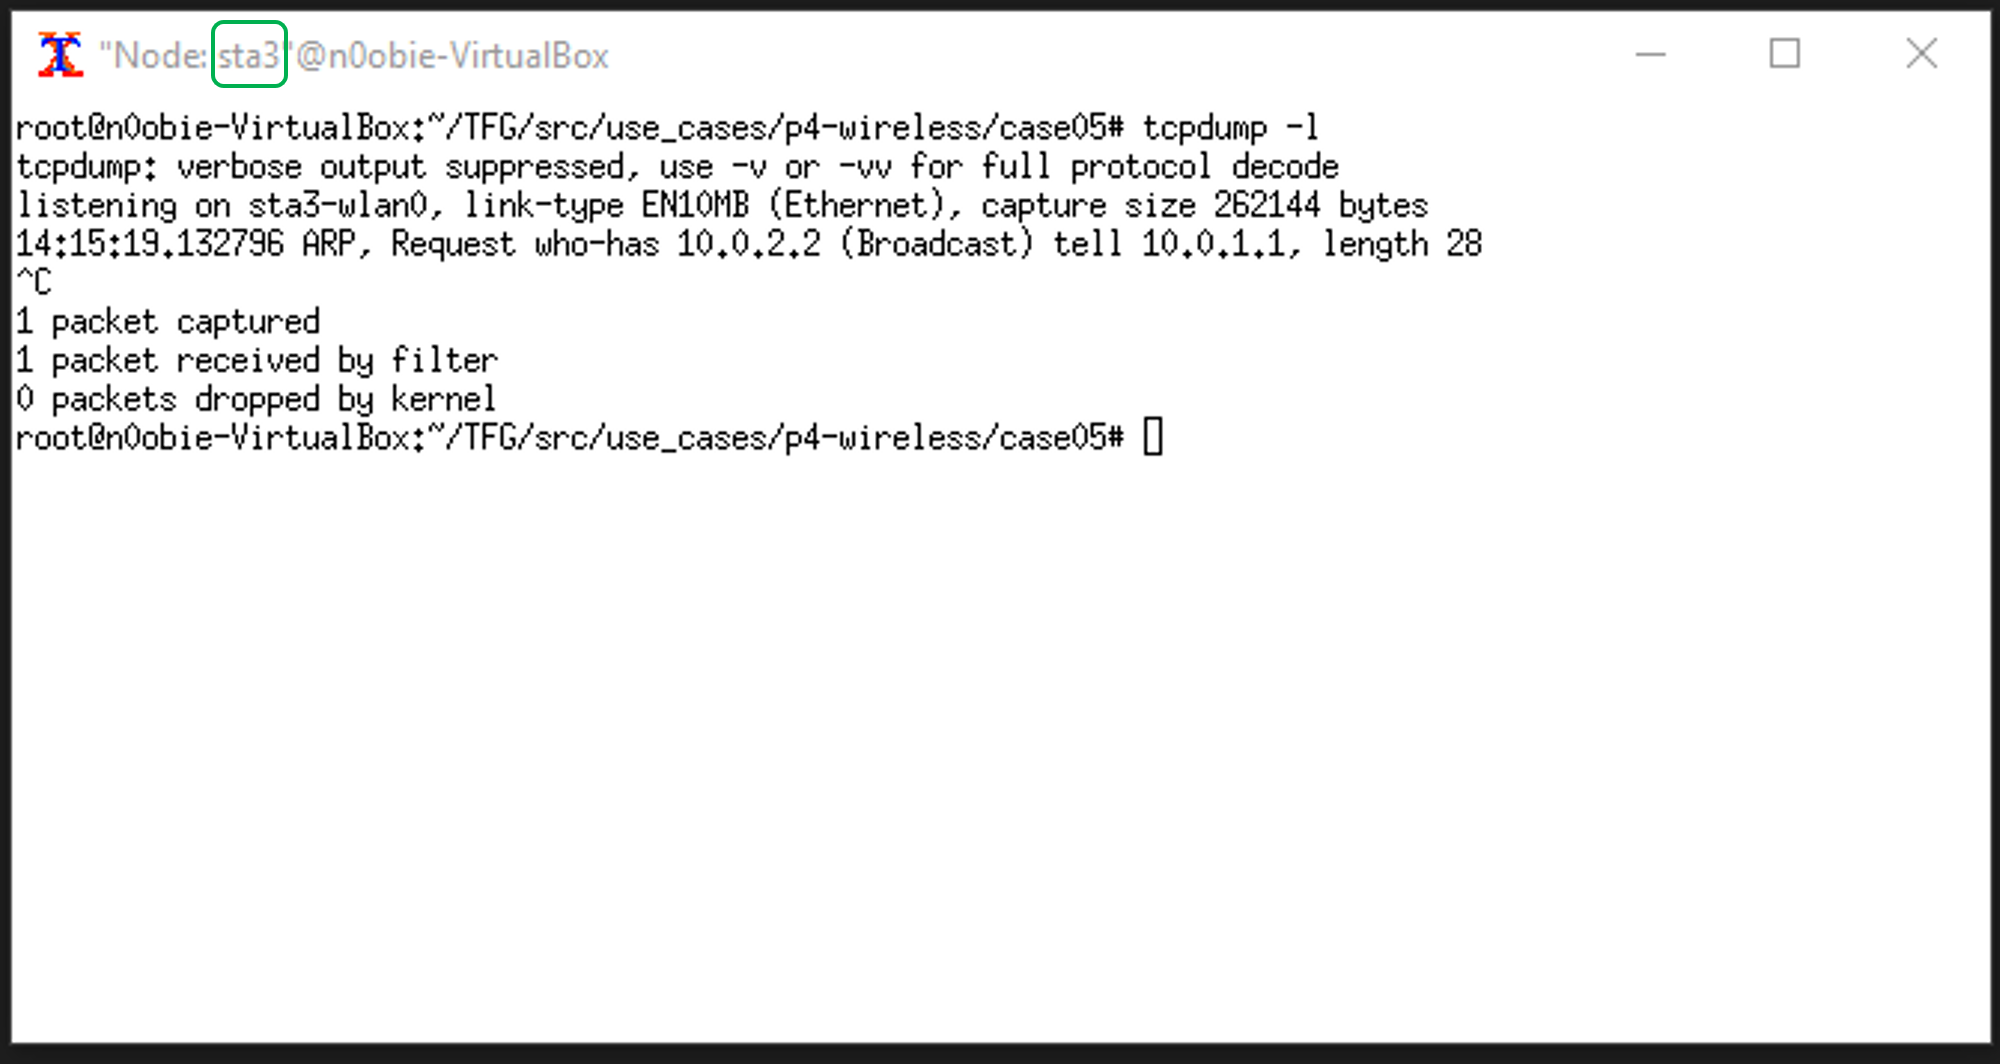
\includegraphics[width=12cm]{archivos/img/dev/p4-wifi/case05/demo_case05_2_edited.png}
        \caption{Escucha con Tcpdump en la estación WiFi sta3}
        \label{fig:case05_p4_wifi_func_list1}
    \end{subfigure}
    \par\bigskip
    \begin{subfigure}[b]{\textwidth}
    	\centering
        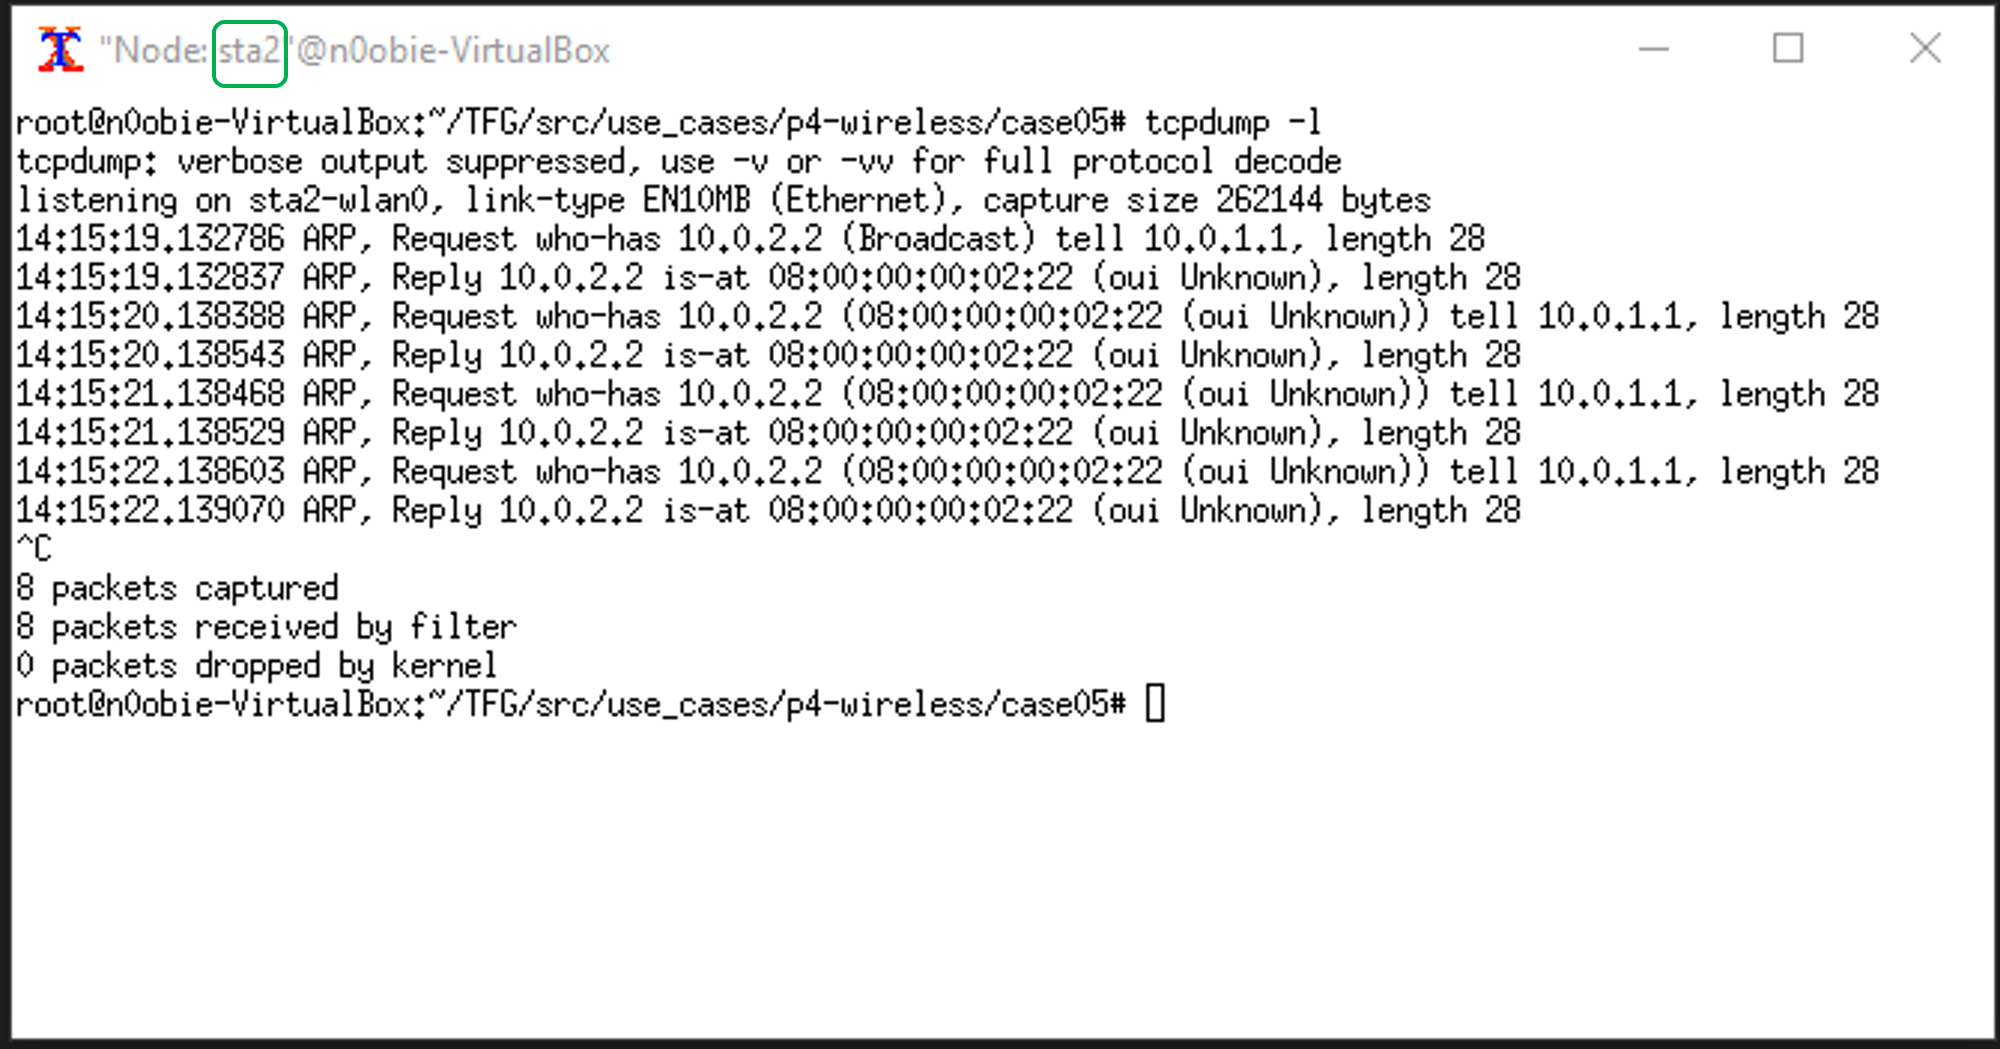
\includegraphics[width=12cm]{archivos/img/dev/p4-wifi/case05/demo_case05_3_edited.png}
        \caption{Escucha con Tcpdump en la estación WiFi sta2}
        \label{fig:case05_p4_wifi_func_list2}
    \end{subfigure}
    
    \caption{Comprobación de funcionamiento del Case05 - P4 Wireless}
    \label{fig:case05_p4_wifi_func1}
\end{figure}